\documentclass{article}
\usepackage{fullpage}
\usepackage[utf8]{inputenc}
\usepackage{pict2e}
\usepackage{amsmath}
\usepackage{enumitem}
\usepackage{eurosym}
\usepackage{mathtools}
\usepackage{amssymb, amsfonts, latexsym, cancel}
\setlength{\parskip}{0.3cm}
\usepackage{graphicx}
\usepackage{fontenc}
\usepackage{slashbox}
\usepackage{setspace}
\usepackage{gensymb}
\usepackage{accents}
\usepackage{adjustbox}
\setstretch{1.35}
\usepackage{bold-extra}
\usepackage[document]{ragged2e}
\usepackage{subcaption}
\usepackage{tcolorbox}
\usepackage{xcolor, colortbl}
\usepackage{wrapfig}
\usepackage{empheq}
\usepackage{array}
\usepackage{parskip}
\usepackage{arydshln}
\graphicspath{ {images/} }
\renewcommand*\contentsname{\color{black}Índice} 
\usepackage{array, multirow, multicol}
\definecolor{lightblue}{HTML}{007AFF}
\usepackage{color}
\usepackage{etoolbox}
\usepackage{listings}
\usepackage{mdframed}
\setlength{\parindent}{0pt}
\usepackage{underscore}
\usepackage{hyperref}
\usepackage{tikz}
\usepackage{tikz-cd}
\usetikzlibrary{shapes, positioning, patterns}
\usepackage{tikz-qtree}
\usepackage{biblatex}
\usepackage{pdfpages}
\usepackage{pgfplots}
\usepackage{pgfkeys}
\addbibresource{biblatex-examples.bib}
\usepackage[a4paper, left=1cm, right=1cm, top=1cm,
bottom=1.5cm]{geometry}
\usepackage{titlesec}
\usepackage{titletoc}
\usepackage{tikz-3dplot}
\usepackage{kbordermatrix}
\usetikzlibrary{decorations.pathreplacing}
\newcommand{\Ej}{\textcolor{lightblue}{\underline{Ejemplo}}}
\setlength{\fboxrule}{1.5pt}

% Configura el formato de las secciones utilizando titlesec
\titleformat{\section}
{\color{red}\normalfont\LARGE\bfseries}
{Tema \thesection:}
{10 pt}
{}

% Ajusta el formato de las entradas de la tabla de contenidos
\addtocontents{toc}{\protect\setcounter{tocdepth}{4}}
\addtocontents{toc}{\color{black}}

\titleformat{\subsection}
{\normalfont\Large\bfseries\color{red}}{\thesubsection)}{1em}{\color{lightblue}}

\titleformat{\subsubsection}
{\normalfont\large\bfseries\color{red}}{\thesubsubsection)}{1em}{\color{lightblue}}

\newcommand{\bboxed}[1]{\fcolorbox{lightblue}{lightblue!10}{$#1$}}
\newcommand{\rboxed}[1]{\fcolorbox{red}{red!10}{$#1$}}

\DeclareMathOperator{\N}{\mathbb{N}}
\DeclareMathOperator{\Z}{\mathbb{Z}}
\DeclareMathOperator{\R}{\mathbb{R}}
\DeclareMathOperator{\Q}{\mathbb{Q}}
\DeclareMathOperator{\K}{\mathbb{K}}
\DeclareMathOperator{\im}{\imath}
\DeclareMathOperator{\jm}{\jmath}
\DeclareMathOperator{\col}{\mathrm{Col}}
\DeclareMathOperator{\fil}{\mathrm{Fil}}
\DeclareMathOperator{\rg}{\mathrm{rg}}
\DeclareMathOperator{\nuc}{\mathrm{nuc}}
\DeclareMathOperator{\dimf}{\mathrm{dimFil}}
\DeclareMathOperator{\dimc}{\mathrm{dimCol}}
\DeclareMathOperator{\dimn}{\mathrm{dimnuc}}
\DeclareMathOperator{\dimr}{\mathrm{dimrg}}
\DeclareMathOperator{\dom}{\mathrm{Dom}}
\DeclareMathOperator{\infi}{\int_{-\infty}^{+\infty}}
\newcommand{\dint}[2]{\int_{#1}^{#2}}

\newcommand{\bu}[1]{\textcolor{lightblue}{\underline{#1}}}
\newcommand{\lb}[1]{\textcolor{lightblue}{#1}}
\newcommand{\db}[1]{\textcolor{blue}{#1}}
\newcommand{\rc}[1]{\textcolor{red}{#1}}
\newcommand{\tr}{^\intercal}

\renewcommand{\CancelColor}{\color{lightblue}}

\newcommand{\dx}{\:\mathrm{d}x}
\newcommand{\dt}{\:\mathrm{d}t}
\newcommand{\dy}{\:\mathrm{d}y}
\newcommand{\dz}{\:\mathrm{d}z}
\newcommand{\dth}{\:\mathrm{d}\theta}
\newcommand{\dr}{\:\mathrm{d}\rho}
\newcommand{\du}{\:\mathrm{d}u}
\newcommand{\dv}{\:\mathrm{d}v}
\newcommand{\tozero}[1]{\cancelto{0}{#1}}
\newcommand{\lbb}[2]{\textcolor{lightblue}{\underbracket[1pt]{\textcolor{black}{#1}}_{#2}}}
\newcommand{\dbb}[2]{\textcolor{blue}{\underbracket[1pt]{\textcolor{black}{#1}}_{#2}}}
\newcommand{\rub}[2]{\textcolor{red}{\underbracket[1pt]{\textcolor{black}{#1}}_{#2}}}

\author{Francisco Javier Mercader Martínez}
\date{}
\title{Cálculo II\\ Tema 3: Cálculo diferencial de funciones de varias variables I}
\everymath{\displaystyle}
\renewcommand{\arraystretch}{1.5}

\begin{document}
\maketitle

\begin{enumerate}[label=\color{red}\textbf{\arabic*)}, leftmargin=*]
	\item \lb{Decir si es o no diferenciable en el punto $(0,0)$ la función real \[ f(x,y)=\begin{cases}
	\dfrac{2xy}{x^2+y^2} & \text{si }(x,y)\neq(0,0)\\
	0 & \text{si }(x,y)=(0,0)
	\end{cases} \]}
	
	Para comprobar si $f(x,y)$ es diferenciable o no en el punto $(0,0)$, lo primero que debemos hacer es comprobar si la función es continua en dicho punto, ya que en caso de no serlo directamente diríamos que es diferenciable.
	\begin{itemize}
	\item Estudio de la continuidad en $(0,0)$:
	
	$\lim_{(x,y)\to(0,0)}\dfrac{2xy}{x^2+y^2}=\left\{\begin{array}{l}
	x=r\cos\theta\\
	y=r\sin\theta
	\end{array}\right\}=\lim_{r\to0}\dfrac{2\cdot r\cos\theta\cdot r\sin\theta}{r^2\cos^2\theta+r^2\sin^2\theta}=\lim_{r\to0}\dfrac{2r^2\cos\theta\sin\theta}{r^2(\lbb{\cos^2\theta+\sin^2\theta}{1})}=\lim_{r\to0}\dfrac{2\cancel{r^2}\cos\theta\sin\theta}{\cancel{r^2}}=2\cos\theta\sin\theta\longrightarrow\nexists\lim$
	
	\end{itemize}
	Como no existe el límite, entonces $f(x,y)$ no es diferenciable en $(0,0)$ y por lo tanto, podemos asegurar que tanto es diferenciable en dicho punto.
	
	\item \lb{Comprobar que la función $f:\R^2\to\R$ definida por $$f(x,y)=\begin{cases}
	x\sin\dfrac{1}{x} & \text{si }(x,y)\neq(0,0)\\
	0 & \text{si }(x,y)=(0,0)
	\end{cases}$$es continua en $(0,0)$, pero no es diferenciable en dicho punto.}
	
	Para comprobar si $f(x,y)$ es diferenciable o no en el punto $(0,0)$, lo primero que debemos hacer es comprobar si la función es continua en dicho punto, ya que en caso de serlo directamente diríamos que no diferenciable.
	
	\begin{itemize}
	\item Estudio de la continuidad en $(0,0)$:
	\[ \lim_{(x,y)\to(0,0)}x\sin\dfrac{1}{x}=\left\{\text{Teorema del Sándwich}\right\}=0 \]
	
	Como el límite coincide con $f(0,0)=0$, la función $f(x,y)$ es continua en $(0,0)$.
	
	\item Comprobar que $f(x,y)$ no es diferenciable en $(0,0)$:
	
	La función $f(x,y)$ es diferenciable en $(0,0)$ si existe un plano tangente que se aproxime localmente a $f(x,y)$. Esto ocurre si: \[ \lim_{(h,k)\to(0,0)}\dfrac{f(h,k)-f(0,0)-\frac{\partial f}{\partial x}(0,0)h-\frac{\partial f}{\partial y}(0,0)k}{\sqrt{h^2+k^2}}=0 \]
	
	$\dfrac{\partial f}{\partial x}(0,0)=\lim_{h\to0}\dfrac{f(h,0)-f(0,0)}{h}=\lim_{h\to0}\dfrac{\cancel{h}\sin\frac{1}{x}-0}{\cancel{h}}=\lim_{h\to0}\sin\dfrac{1}{h}$
	
	El término $\sin\dfrac{1}{x}$ oscila entre -1 y 1 de manera no convergente cuando $h\to0$, por lo que este límite no existe. Por lo tanto, la función no es diferenciable en $(0,0)$.
	\end{itemize}
	
	\item \lb{Estudiar la continuidad y la diferenciabilidad de la función $f:\R^2\to\R$ definida por \[ f(x,y)=\begin{cases}
	\dfrac{xy^2}{x^2+y^2} & \text{si }(x,y)\neq(0,0)\\
	0 & \text{si }(x,y)=(0,0)
	\end{cases} \] Calcular su derivada direccional de cualquier vector $v=(v_1,v_2)$ en el punto $(0,0)$.}
	
	\begin{itemize}
	\item Estudio de la continuidad en el punto $(0,0)$:
	
	$\lim_{(x,y)\to(0,0)}\dfrac{xy^2}{x^2+y^2}=\left\{\begin{array}{l}
	x=r\cos\theta\\
	y=r\sin\theta
	\end{array}\right\}=\lim_{r\to0}\dfrac{r\cos\theta r^2\sin^2\theta}{\lbb{r^2\cos^2\theta+r^2\sin^2\theta}{r^2}}=\lim_{r\to0}\dfrac{r^{\cancel{3}}\cos\theta\sin^2\theta}{\cancel{r^2}}=\lim_{r\to0}r\cos\theta\sin^2\theta=0$
	
	Como el límite coincide con $f(0,0)=0$, la función $f(x,y)$ es continua en dicho punto.
	
	\item Comprobar que $f(x,y)$ es diferenciable en $(0,0)$:
	
	Para verificar la diferenciabilidad en $(0,0)$, usando el criterio de que la función es diferenciable si existe un plano tangente local, lo que requiere que: \[ \lim_{(h,k)\to(0,0)}\dfrac{\left|f(h,k)-f(0,0)-\frac{\partial f}{\partial x}(0,0)h-\frac{\partial f}{\partial y}(0,0)k\right|}{\sqrt{h^2+k^2}}=0 \]
	Esto requiere calcular las derivadas parciales en $(0,0)$.
	
	$\begin{array}{l}
	\dfrac{\partial f}{\partial x}(0,0)=\lim_{h\to0}\dfrac{f(h,0)-f(0,0)}{h}=\lim_{h\to0}\dfrac{0-0}{h}=0\\
	\dfrac{\partial f}{\partial y}(0,0)=\lim_{k\to0}\dfrac{f(0,k)-f(0,0)}{k}=\lim_{k\to0}\dfrac{0-0}{k}=0
	\end{array}$
	
	Si $f(x,y)$ fuera diferenciable, se debería cumplir:
	
	\[ \begin{aligned}
	\lim_{(x,y)\to(0,0)}\dfrac{f(h,k)-0}{\sqrt{h^2+k^2}}&=\left\{\begin{array}{l}
	h=r\cos\theta\\
	k=r\sin\theta
	\end{array}\right\}=\lim_{r\to0}\dfrac{\frac{r\cos\theta r^{2}\sin^{2}\theta}{r^2\cos^2\theta+r^2\sin^{2}\theta}}{\sqrt{\lbb{r^{2}\cos^{2}\theta+r^{2}\sin^2\theta}{r^{2}}}}=\lim_{r\to0}\dfrac{\cancel{r^{3}}\cos\theta\sin^{2}\theta}{\cancel{r^{3}}}\\
	& =\cos\theta\sin^{2}\theta\longrightarrow\nexists\lim
	\end{aligned} \]
	
	El término $\cos\theta\sin^{2}\theta$ depende de $\theta$, lo que implica que el límite no existe uniformemente. Por lo tanto, la función no es diferenciable en $(0,0)$.
	
	\item Derivada direccional en $(0,0)$:
	
	La derivada direccional en la dirección $\mathrm{v}=(v_1,v_2)$ está dada por:
	\[ \begin{aligned}
	D_{\mathrm{v}}f(0,0)&=\lim_{t\to0}\dfrac{f(tv_1,tv_2)-f(0,0)}{t}=\lim_{t\to0}\dfrac{\dfrac{(tv_{1})(tv_{2})^{2}}{(tv_{1})^{2}+(tv_{2})^{2}}-0}{t}=\lim_{t\to0}\dfrac{\dfrac{t^{3}v_1v_2^2}{t^{2}(v_1^2+v_2^2)}}{t}\\
	&=\lim_{t\to0}\dfrac{\cancel{t^{3}}v_1v_2^2}{\cancel{t^{3}}(v_1^2+v_2^2)}=\dfrac{v_1v_2^2}{v_1^2+v_2^2}
	\end{aligned} \]
	
	La derivada direccional no siempre es cero, ya que depende de los valores de $v_1$ y $v_2$.
	\end{itemize}
	
	\item \lb{Sea $f:\R^{2}\to\R$ definida por \[ f(x,y)=\begin{cases}
	\dfrac{xy^{2}}{x^{2}+y^{4}} & \text{si }(x,y)\neq(0,0)\\
	0 & \text{si }(x,y)=(0,0)
	\end{cases} \]Comprobar que $f$ tiene derivada direccional respecto de cualquier vector de $\R^2$ en el punto $(0,0)$, pero $f$ no es derivable en dicho punto.}
	
\begin{itemize}
\item Derivada direccional en $(0,0)$:

	La derivada direccional de $f(x,y)$ en la dirección de un vector $\mathrm{v}=(v_1,v_2)\in\R^2$ se define como:
	\[ \begin{aligned}
	D_{\mathrm{v}}f(0,0)&=\lim_{t\to0}\dfrac{f(tv_1,tv_2)-f(0,0)}{t}=\lim_{t\to0}\dfrac{f(tv_1,tv_2)}{t}=\lim_{t\to0}\dfrac{\dfrac{(tv_1)(tv_2)^{2}}{(tv_1)^{2}+(tv_2)^{4}}}{t}=\lim_{t\to0}\dfrac{\dfrac{t^{3}v_1v_2^{2}}{t^2v_1^2+t^4v_2^4}}{t}\\
	&=\lim_{t\to0}\dfrac{t^{\cancel{3}}v_1v_2^2}{\cancel{t}(t^2v_1^2+t^4v_2^4)}=\lim_{t\to0}\dfrac{\cancel{t^{2}}(v_1v_2^2)}{\cancel{t^{2}}(v_1^2+t^2v_2^4)}=\lim_{t\to0}\dfrac{v_1v_2^2}{v_2^2+\tozero{t^2v_2^4}}=\dfrac{\cancel{v_1}v_2^2}{v_1^{\cancel{2}}}=\dfrac{v_2^2}{v_1}
	\end{aligned} \]
	
	La derivada direccional existe para cualquier vector $\mathrm{v}=(v_1,v_2)$ y está dada por \[ D_{\mathrm{v}}f(0,0)=\begin{cases}
	\dfrac{v_2^2}{v_1}, & \text{si }v_1\neq0\\
	0 & \text{si }v_1=0\text{ y }v_2=0
	\end{cases} \]
	\item Diferenciabilidad de $f(x,y)$ en $(0,0)$:
	
	La función $f(x,y)$ es diferenciable en $(0,0)$ si existe: \[ \lim_{(h,k)\to(0,0)}\dfrac{\left|f(h,k)-f(0,0)-\frac{\partial f}{\partial x}(0,0)h-\frac{\partial f}{\partial y}(0,0)k\right|}{\sqrt{h^2+k^2}}=0 \]
	
	Esto requiere calcular las derivadas parciales en $(0,0)$.
	
	$\begin{array}{l}
	\dfrac{\partial f}{\partial x}=\lim_{h\to0}\dfrac{f(h,0)- f(0,0)}{h}=\lim_{h\to0}\dfrac{0-0}{h}=0\\
	\dfrac{\partial f}{\partial y}=\lim_{k\to0}\dfrac{f(0,k)- f(0,0)}{k}=\lim_{k\to0}\dfrac{0-0}{k}=0\\
	\end{array}$
	
	Si $f(x,y)$ fuera diferenciable en $(0,0)$, las derivadas direccionales serían consistentes con las derivadas parciales. Sin embargo, observamos que \[ D_{\mathrm{v}}f(0,0)=\dfrac{v_2^2}{v_1},\quad\text{si }v_1\neq0, \]y esto depende de la dirección $\mathrm{v}=(v_1,v_2)$, lo cual indica que $f(x,y)$ no puede aproximarse localmente por una aplicación lineal.
	
	La función no es diferenciable en $(0,0)$ porque las derivadas direccionales no son consistentes con una aproximación lineal.
\end{itemize}

\item \lb{Calcular las derivadas parciales de la función \[ f(x,y)=x^{2}\tan\dfrac{y^2}{x^2+y^2} \]definida para todo punto de $\R^2\backslash\{(0,0)\}$, y comprobar que \[ xD_1f(x,y)+yD_2f(x,y)=2f(x,y) \]}

Denotamos $u=\dfrac{y^{2}}{x^2+y^2}$. Entonces: \[ f(x,y)=x^{2}\tan(u) \]

$\dfrac{\partial f}{\partial x}=2x\tan(u)+x^{2}(\tan^{2}(u)+1)\dfrac{\partial u}{\partial x}=2x\tan(u)+x^{2}(\tan^{2}(u)+1)\cdot\left(-\dfrac{2xy^{2}}{(x^{2}+y^{2})^{2}}\right)$

$\begin{aligned}
\dfrac{\partial f}{\partial y}&=x^{2}(\tan^{2}+1)\cdot\dfrac{\partial u}{\partial y}=x^{2}(\tan^{2}(u)+1)\cdot\left(\dfrac{2y(x^{2+y^{2}-y^{2}\cdot2y})}{(x^{2}+y^{2})^{2}}\right)=x^{2}(\tan^{2}(u)+1)\cdot\left(\dfrac{2x^{2}y+\cancel{2y^{3}}-\cancel{2y^{3}}}{(x^{2}+y^{2})^{2}}\right)\\
&=x^{2}(\tan^{2}(u)+1)\cdot\left(\dfrac{2x^{2}y}{(x^{2}+y^{2})^{2}}\right)
\end{aligned}$

$\begin{aligned}
xD_1f(x,y)+yD_2f(x,y)&=x\cdot\left[2x\tan(u)+x^{2}(\tan^{2}(u)+1)\cdot\left(-\dfrac{2xy^{2}}{(x^{2}+y^{2})^{2}}\right)\right]+y\cdot\left[x^{2}(\tan^{2}(u)+1)\cdot\left(\dfrac{2x^{2}y}{(x^{2}+y^{2})^{2}}\right)\right]\\
&=2x^{2}\tan(u)-\cancel{\dfrac{2x^{4}y^{2}}{(x^{2}+y^{2})^{2}}\cdot(\tan^{2}(u)+1)}+\cancel{\dfrac{2x^{4}y^{2}}{(x^{2}+y^{2})^{2}}\cdot(\tan^{2}(u)+1)} = 2x^{2}\tan(u)
\end{aligned}$

Por lo tanto: \[ x\cdot\dfrac{\partial f}{\partial x}+y\cdot\dfrac{\partial f}{\partial y}=2\cdot f(x,y) \]

\item \lb{Calcular las derivadas parciales de la función \[ f(x,y)=\dfrac{\sqrt{x}+\sqrt{y}}{x+y} \]definida en el conjunto $\{(x,y):x>0,y>0\}$, y comprobar que \[ xD_1f(x,y)+yD_2f(x,y)=-\dfrac{1}{2}f(x,y) \]}

$\dfrac{\partial f}{\partial x}=\dfrac{\dfrac{1}{2\sqrt{x}}(x+y)-(\sqrt{x}+\sqrt{y})\cdot1}{(x+y)^{2}}=\dfrac{\dfrac{1}{2\sqrt{x}}(x+y)-(\sqrt{x}+\sqrt{y})}{(x+y)^{2}}$

$\dfrac{\partial f}{\partial y}=\dfrac{\dfrac{1}{2\sqrt{y}}(x+y)-(\sqrt{x}+\sqrt{y})\cdot1}{(x+y)^{2}}=\dfrac{\dfrac{1}{2\sqrt{y}}(x+y)-(\sqrt{x}+\sqrt{y})}{(x+y)^{2}}$

$\begin{aligned}
x\cdot\dfrac{\partial f}{\partial y}+y\cdot\dfrac{\partial f}{\partial y}&=x\cdot\dfrac{\dfrac{1}{2\sqrt{x}}(x+y)-(\sqrt{x}+\sqrt{y})}{(x+y)^{2}}+y\cdot\dfrac{\dfrac{1}{2\sqrt{y}}(x+y)-(\sqrt{x}+\sqrt{y})}{(x+y)^{2}}\\
&=\dfrac{x\cdot\left(\dfrac{1}{2\sqrt{x}}(x+y)-(\sqrt{x}+\sqrt{y})\right)+y\cdot\left(\dfrac{1}{2\sqrt{y}}(x+y)-(\sqrt{x}+\sqrt{y})\right)}{(x+y)^{2}}\\
& =\dfrac{\dfrac{\sqrt{x}}{2}(x+y)-x(\sqrt{x}+\sqrt{y})+\dfrac{\sqrt{y}}{2}(x+y)-y(\sqrt{x}+\sqrt{y})}{(x+y)^2}\\
&=\dfrac{\dfrac{1}{2}(\sqrt{x}+\sqrt{y})(x+y)-(\sqrt{x}+\sqrt{y})(x+y)}{(x+y)^{2}}=\dfrac{\left(\dfrac{1}{2}-1\right)(\sqrt{x}+\sqrt{y})\cancel{(x+y)}}{(x+y)^{\cancel{2}}}=-\dfrac{1}{2}\cdot\dfrac{\sqrt{x}+\sqrt{y}}{x+y}
\end{aligned}$

Por lo tanto: \[ x\cdot\dfrac{\partial f}{\partial x}+y\cdot\dfrac{\partial f}{\partial y}=-\dfrac{1}{2}\cdot f(x,y) \]

\item \lb{Calcular las derivadas parciales de la función \[ f(x,y)=y\cdot\log\dfrac{x^{3}y}{x^{2}+y^{2}} \]definida en el conjunto $\{(x,y):x>0,y>0\}$, y calcular su diferencial en el punto $(1,1)$.}

$\begin{aligned}
\dfrac{\partial f}{\partial x}&=y\cdot\dfrac{1}{\dfrac{x^{3}y}{x^{2}+y^{2}}}\cdot\dfrac{3x^{2}y\cdot(x^{2}+y^{2})-x^{3}y\cdot2x}{(x^{2}+y^{2})^{2}}=\dfrac{\cancel{x^{2}+y^{2}}}{x^{3}y}\cdot\dfrac{3x^{4}y+3x^{2}y^{3}-2x^{4}y}{(x^{2}+y^{2})^{\cancel{2}}}\cdot y\\
&=y\cdot\dfrac{x^{4}y+3x^{2}y^{3}}{x^{3}y(x^{2}+y^{2})}=\cancel{y}\cdot\dfrac{x^{4}y+3x^{2}y^{3}}{x^{5}\cancel{y}+x^{3}y^{\cancel{3}}}=\dfrac{x^{4}y+3x^{2}y^{3}}{x^{5}+x^{3}y^{2}}
\end{aligned}$

$\dfrac{\partial f}{\partial y}=1\cdot\log\dfrac{x^{3}y}{x^{2}+y^{2}}+\cancel{y}\cdot\dfrac{\cancel{x^{2}+y^{2}}}{\cancel{x^{3}y}}\cdot\dfrac{\cancel{x^{3}}(x^{2}+y^{2})-\cancel{x^{3}}y\cdot2y}{(x^{2}+y^{2})^{\cancel{2}}}=\log\dfrac{x^{3}y}{x^{2}+y^{2}}+\dfrac{x^{2}+y^{2}-2y^{2}}{x^{2}+y^{2}}=\log\dfrac{x^{3}y}{x^{2}+y^{2}}+\dfrac{x^{2}-y^{2}}{x^{2}+y^{2}}$

$\begin{array}{l}
\dfrac{\partial f}{\partial x}(1,1)=\dfrac{1^{3}\cdot1+3\cdot1^{2}\cdot1^{3}}{1^{5}+1^{3}\cdot y^{2}}=\dfrac{4}{2}=2\\
\dfrac{\partial f}{\partial y}(1,1)=\log\dfrac{1^{3}\cdot 1}{1^{2}+1^{2}}+\tozero{\dfrac{1^{2}-1^{2}}{1^{2}+1^{2}}}=\log\dfrac{1}{2}
\end{array}$

El diferencial en $(1,1)$ es: \[ \mathrm{d}f=\dfrac{\partial f}{\partial x}\dx+\dfrac{\partial f}{\partial y}(1,1)\dy=2\dx+\log\dfrac{1}{2}\dy \]

\item \lb{Calcular las derivadas parciales de la función \[ f(x,y)=\sqrt{xy+\dfrac{x}{y}} \]definida en el conjunto $\{(x,y):x>0,y>0\}$, y calcular su diferencial en el punto $(2,1)$.}

$\begin{array}{l}
\dfrac{\partial f}{\partial x}=\dfrac{1}{2\sqrt{xy+\frac{x}{y}}}\cdot\left(y+\dfrac{1}{y}\right)\longrightarrow\dfrac{\partial f}{\partial x}(2,1)=\dfrac{1}{2\sqrt{2\cdot 1+\frac{2}{1}}}\cdot\left(1+\dfrac{1}{1}\right)=\dfrac{2}{2\sqrt{4}}=\dfrac{1}{2}\\
\dfrac{\partial f}{\partial y}=\dfrac{1}{2\sqrt{xy+\frac{x}{y}}}\cdot\left(x-\dfrac{y}{x^{2}}\right)\longrightarrow\dfrac{\partial f}{\partial y}(2,1)=\dfrac{1}{2\sqrt{2\cdot1+\frac{2}{1}}}\cdot\left(2-\dfrac{2}{1}\right)=0\\
\end{array}$

El diferencial en $(2,1)$ es: \[ \mathrm{d}f=\dfrac{\partial f}{\partial x}(2,1)\dx+\dfrac{\partial f}{\partial y}(2,1)\dy=\dfrac{1}{2}\dx \]

\item \lb{Dada la función $\vec{f}:\R^{2}\to\R^{2}$ definida por \[ \vec{f}(x,y)=\left(x^{4}+y^{3},x^{2}y^{2}-3y^{2}\right) \]formar su matriz jacobiana en el punto $(1,1)$. Comprobar que $\vec{f}$ es diferenciable en dicho punto y calcular su diferencial.}

$f(x,y)=\left(x^{4}+y^{3},x^{2}y^{2}-3y^{2}\right)=\begin{cases}
f_1(x,y)=x^{4}+y^{3}\\
f_2(x,y)=x^{2}y^{2}-3y^{2}
\end{cases}$

$J(f)=\begin{pmatrix}
\dfrac{\partial f_1}{\partial x} & \dfrac{\partial f_1}{\partial y} \\
\dfrac{\partial f_{2}}{\partial x} & \dfrac{\partial f_2}{\partial y}
\end{pmatrix}=\begin{pmatrix}
4x^{3} & 3y^2 \\
 2xy^{2} & 2x^{2}y-6y
\end{pmatrix}\longrightarrow J(1,1)=\begin{pmatrix}
4 & 3 \\
2 & -4
\end{pmatrix}$

Como todas las funciones son continuas y con derivadas primeras continuas, podemos asegurar que es diferenciable.

Su diferencial, al ser una función vectorial, vendrá dado por:
\[ \begin{aligned}
\mathrm{d}f(P)(h,k)&=J(f)(P)(h,k)=\mathrm{d}f(1,1)(h,k)=J(f)(1,1)\binom{h}{k}\\
&=\begin{pmatrix}
4 & 3 \\
2 & -4
\end{pmatrix}\cdot\begin{pmatrix}
h\\
k
\end{pmatrix}=\begin{pmatrix}
4h+3k\\
2h-4k
\end{pmatrix}\longrightarrow \mathrm{d}f(1,1)(h,k)=(4h+3k,\,2h-4k)
\end{aligned} \]

\item \lb{Dada la función $\vec{f}:\R^{2}\to\R^{3}$ definida por \[ \vec{f}(x,y)=(x\cos y,x\sin y,x\cos y\sin y) \]formar su matriz jacobiana en el punto $\left(\pi,\dfrac{\pi}{2}\right)$. Comprobar que $\vec{f}$ es diferenciable en dicho punto y calcular su diferencial.}

$\vec{f}(x,y)=(x\cos y,x\sin y,x\cos y\sin y)=\begin{cases}
f_{1}(x,y)=x\cos y\\
f_{2}(x,y)=x\sin y\\
f_{3}(x,y)=x\cos y\sin y
\end{cases}$

$J(f)=\begin{pmatrix}
\dfrac{\partial f_{1}}{\partial x} & \dfrac{\partial f_1}{\partial y} \\ 
\dfrac{\partial f_{2}}{\partial x} & \dfrac{\partial f_2}{\partial y} \\ 
\dfrac{\partial f_{3}}{\partial x} & \dfrac{\partial f_3}{\partial y} \\ 
\end{pmatrix}=\begin{pmatrix}
\cos y & -x\sin y \\ 
\sin y & x\cos y \\ 
\cos y\sin y & x(-\sin^{2}y+\cos^{2}y)
\end{pmatrix}\longrightarrow J(f)\left(\pi,\dfrac{\pi}{2}\right)=\begin{pmatrix}
0 & -\pi \\ 
1 & 0 \\ 
0 & -\pi
\end{pmatrix}  $

Como todas las funciones son continuas y con derivadas primeras continuas, entonces podemos asegurar que todas las funciones coordenada son $C^{1}$, por lo tanto la función $\vec{f}(x,y)$ es también $C^{1}$ y también es diferenciable.

\[ \begin{aligned}
\mathrm{d}f(P)(h,k)&=J(f)(P)(h,k)=\mathrm{d}f\left(\pi,\dfrac{\pi}{2}\right)(h,k)=J(f)\left(\pi,\dfrac{\pi}{2}\right)\binom{h}{k}\\
&=\begin{pmatrix}
0 & -\pi \\ 
1 & 0 \\ 
0 & -\pi
\end{pmatrix}\cdot\begin{pmatrix}
h\\
k
\end{pmatrix}=\left(-\pi k,\,h,\,-\pi k\right)\longrightarrow \mathrm{d}f\left(\pi,\dfrac{\pi}{2}\right)(h,k)=\left(-\pi k,\,h,\,-\pi k\right)
\end{aligned} \]

\item \lb{Comprobar que la función $\vec{f}:\R^{3}\to\R^{3}$ definida por \[ \vec{f}(x,y,z)=(x^{2}+yz-z^{2},\, xy-xz+2z^{2},\, xyz) \]es diferenciable en todo punto de $\R^{3}$ y calcularla en el punto $(3,2,1)$.}

$\vec{f}(x,y,z)=(x^{2}+yz-z^{2},\, xy-xz+2z^{2},\, xyz)=\begin{cases}
f_1(x,y,z)=x^{2}+yz-z^{2}\\
f_2(x,y,z)=xy-xz+2z^{2}\\
f_3(x,y,z)=xyz
\end{cases}$

Como todas las funciones son continuas y con derivadas primeras continuas, entonces podemos asegurar que son diferenciables, por consecuencia, $\vec{f}(x,y,z)$ también es diferenciable.

$J(f)=\begin{pmatrix}
\dfrac{\partial f_{1}}{\partial x} & \dfrac{\partial f_1}{\partial y} & \dfrac{\partial f_1}{\partial z} \\ 
\dfrac{\partial f_{2}}{\partial x} & \dfrac{\partial f_2}{\partial y} & \dfrac{\partial f_2}{\partial z} \\ 
\dfrac{\partial f_{3}}{\partial x} & \dfrac{\partial f_3}{\partial y} & \dfrac{\partial f_3}{\partial z} \\ 
\end{pmatrix}=\begin{pmatrix}
2x & z & y-2z \\
y-z & x & -x+4z \\
yz & xz & xy
\end{pmatrix}\longrightarrow J(f)(3,2,1)=\begin{pmatrix}
6 & 1 & 0 \\
1 & 3 & 1 \\
2 & 3 & 6
\end{pmatrix}$

Su diferencial al ser una función vectorial, vendrá dado por:
\[ \begin{aligned}
\mathrm{d}f(P)(h,k,j)&=J(f)(P)(h,k,j)\longrightarrow\mathrm{d}f(3,2,1)(h,k,j)=J(f)(3,2,1)\begin{pmatrix}
h\\
k\\
j
\end{pmatrix}\\
&=\begin{pmatrix}
6 & 1 & 0 \\
1 & 3 & 1 \\
2 & 3 & 6
\end{pmatrix}\cdot\begin{pmatrix}
h\\
k\\
j
\end{pmatrix}=(6h+k,\, h+3k+j,\, 2h+3k+6j)\\
&\longrightarrow \mathrm{d}f(3,2,1)(h,k,j)=(6h+k,\, h+3k+j,\, 2h+3k+6j)
\end{aligned} \]

\item \lb{Calcular la matriz jacobiana de las siguientes funciones:}
\begin{enumerate}[label=\color{red}\textbf{\alph*)}]
	\item $\db{f(x,y,z)=x^{y+z}}$
	
	$J(f)=\begin{pmatrix}
	\dfrac{\partial f}{\partial x} & \dfrac{\partial f}{\partial y} & \dfrac{\partial f}{\partial z}
	\end{pmatrix}=\begin{pmatrix}
	(y+z)x^{y+z-1} & x^{y+z}\cdot\ln(x) & x^{y+z}\cdot\ln(x)
	\end{pmatrix}$
	
	\item $\db{f(x,y,z)=x^{y^{z}}}$
	
	$J(f)=\begin{pmatrix}
		\dfrac{\partial f}{\partial x} & \dfrac{\partial f}{\partial y} & \dfrac{\partial f}{\partial z}
		\end{pmatrix}=\begin{pmatrix}
		y^{z}\cdot x^{y^{z}-1} & x^{y^{z}}\cdot\ln(x)\cdot z\cdot y^{z-1} & x^{y^{z}}\cdot\ln(x)\cdot y^{z}\cdot\ln(y)
		\end{pmatrix}$
		
	\item $\db{f(x,y,z)=\sin(x\sin(y\sin z))}$
	
	$J(f)=\begin{pmatrix}
			\dfrac{\partial f}{\partial x} & \dfrac{\partial f}{\partial y} & \dfrac{\partial f}{\partial z}
			\end{pmatrix}\\=
			\left(\cos(x\sin(y\sin z))\cdot(\sin(y\sin z)), \cos(x\sin(y\sin z))\cdot x\cdot\cos(y\sin z)\cdot\sin z , \cos(x\sin(y\sin z))\cdot x\cdot \cos(y\sin z)\cdot y\cos z\right)$
			
	\item $\db{\vec{f}(x,y)=(\sin(xy), \sin(x\sin y), x^{4})}$
	
	$J(f)=\begin{pmatrix}
	\dfrac{\partial f_1}{\partial x} & \dfrac{\partial f_1}{\partial y}\\
	\dfrac{\partial f_2}{\partial x} & \dfrac{\partial f_2}{\partial y}\\
	\dfrac{\partial f_3}{\partial x} & \dfrac{\partial f_3}{\partial y}\\
	\end{pmatrix}=\begin{pmatrix}
	\cos(xy)\cdot y & \cos(x,y)\cdot x\\
	\cos(x\sin y)\cdot\sin y & \cos(x\sin y)\cdot x\cdot\cos(y)\\
	4x^{3} & 0
	\end{pmatrix}$
\end{enumerate}

\item \lb{Sea $f:\R^{2}\to\R^{2}$ definida por \[ f(x,y)=\begin{cases}
\left(x^{2}+x^{2}\sin\dfrac{1}{x},\:y\right) & \text{si }(x,y)\neq(0,0)\\
(0,y) & \text{si }(x,y)=(0,y)
\end{cases} \]Comprobar que $f$ es diferenciable.}

$f(x,y)=\begin{cases}
\left(x^{2}+x^{2}\sin\dfrac{1}{x},\:y\right) & \text{si }x\neq0\\
(0,y) & \text{si }x=0
\end{cases}$
\begin{itemize}
\item Caso $x\neq0$:

La función es $C^{1}$ en esta región porque las funciones $x^{2},\,\sin\dfrac{1}{x}$, y $y$ son derivables, y no hay discontinuidades cuando $x\neq0$. Por lo tanto, $f$ es diferenciable en esta región.

\item Caso $x=0$:

Cuando $x=0$, la función se define como \[ f(x,y)=(0,y) \]En este caso, debemos comprobar la diferenciabilidad en el punto $(0,y_0)$ para cualquier $y_0$. Empezamos calculando las derivadas parciales.
\begin{itemize}[label=\textbullet]
	\item Primera componente $f_1(x,y)$: \[ f_1(x,y)=\begin{cases}
	x^{2}+x^{2}\sin\dfrac{1}{x} & \text{si }x\neq0\\
	0 & \text{si }x=0
	\end{cases} \] Para $x\neq0$, la derivada parcial respecto a $x$ es: \[ \dfrac{\partial f_1}{\partial x}=2x+2x\sin\dfrac{1}{x}+\cancel{x^{2}}\cos\dfrac{1}{x}\cdot\left(-\dfrac{1}{\cancel{x^{2}}}\right)=2x+2x\sin\dfrac{1}{x}-\cos\dfrac{1}{x} \]
	\item Segunda componente $f_2(x,y)$: \[ f_2(x,y)=y \] La derivada parcial respecto a $y$ es constante, y vale $1$ en todo $\R^{2}$.
\end{itemize}
En el caso $x=0$, el comportamiento de $\dfrac{\partial f_1}{\partial x}$ es consistente con la definición y es continuo. Por lo tanto, todas las derivadas son continuas en $(0,y_0)$.

Dado que la función $f(x,y)$ es de clase $C^{1}$ en $x\neq0$ y las derivadas parciales son continuas en $x=0$, podemos concluir que $f(x,y)$ es diferenciable en $\R^{2}$.
\end{itemize}

\item \lb{Sabiendo que $f(x,y)=\sqrt{\log(xy)+\arcsin\dfrac{y}{x}}$, calcular \[ xf(x,y)D_1f(x,y)+yf(x,y)D_2f(x,y). \]}

$\begin{array}{l}
\dfrac{\partial f}{\partial x}=\dfrac{1}{2\sqrt{\log(xy)+\arcsin\dfrac{y}{x}}}\cdot\left(\dfrac{1}{x\cancel{y}}\cdot \cancel{y}+\dfrac{1}{\sqrt{1-\dfrac{y^{2}}{x^{2}}}}\cdot\left(-\dfrac{y}{x^{2}}\right)\right)\\
\dfrac{\partial f}{\partial y}=\dfrac{1}{2\sqrt{\log(xy)+\arcsin\dfrac{y}{x}}}\cdot\left(\dfrac{1}{\cancel{x}y}\cdot\cancel{x}+\dfrac{1}{\sqrt{1-\dfrac{y^{2}}{x^{2}}}}\cdot\dfrac{1}{x}\right)
\end{array}$

$\begin{aligned}
xf(x,y)D_1f(x,y)+yf(x,y)D_2f(x,y)=&x\cdot\cancel{\sqrt{\log(xy)+\arcsin\dfrac{y}{x}}}\cdot\dfrac{1}{2\cancel{\sqrt{\log(xy)+\arcsin\dfrac{y}{x}}}}\left(\dfrac{1}{x}-\dfrac{y}{x^{2}\sqrt{1-\dfrac{y^{2}}{x^{2}}}}\right)\\
&+y\cdot\cancel{\sqrt{\log(xy)+\arcsin\dfrac{y}{x}}}\cdot\dfrac{1}{2\cancel{\sqrt{\log(xy)+\arcsin\dfrac{y}{x}}}}\left(\dfrac{1}{y}+\dfrac{1}{x\sqrt{1-\dfrac{y^{2}}{x^{2}}}}\right)\\
=&\dfrac{1}{2}-\cancel{\dfrac{y}{2x\sqrt{1-\dfrac{y^{2}}{x^{2}}}}}+\dfrac{1}{2}+\cancel{\dfrac{y}{2x\sqrt{1-\dfrac{y^{2}}{x^{2}}}}}=1
\end{aligned}$

\item \lb{Sabiendo que $f(x,y)=\sin\dfrac{2x+y}{2x-y}$, calcular \[ xD_1f(x,y)+yD_2f(x,y). \]}

$\begin{array}{l}
\dfrac{\partial f}{\partial x}=\cos\dfrac{2x+y}{2x-y}\cdot\left(\dfrac{2\cdot(2x-y)-(2x+y)\cdot2}{(2x-y)^{2}}\right)=\cos\dfrac{2x+y}{2x-y}\cdot\left(\dfrac{\cancel{4x}-2y-\cancel{4x}-2y}{(2x-y)^{2}}\right)=\cos\dfrac{2x+y}{2x-y}\cdot\left(\dfrac{-4y}{(2x-y)^{2}}\right)\\
\dfrac{\partial f}{\partial y}=\cos\dfrac{2x+y}{2x-y}\cdot\left(\dfrac{1\cdot(2x-y)-(2x+y)\cdot(-1)}{(2x-y)^{2}}\right)=\cos\dfrac{2x+y}{2x-y}\cdot\left(\dfrac{2x-\cancel{y}+2x+\cancel{y}}{(2x-y)^{2}}\right)=\cos\dfrac{2x+y}{2x-y}\cdot\left(\dfrac{4x}{(2x-y)^{2}}\right)
\end{array}$

$\begin{aligned}
xD_1f(x,y)+yD_2f(x,y)&=x\cdot\cos\dfrac{2x+y}{2x-y}\cdot\left(\dfrac{-4y}{(2x-y)^{2}}\right)+y\cdot\cos\dfrac{2x+y}{2x-y}\cdot\left(\dfrac{4x}{(2x-y)^{2}}\right)\\
&=\cos\dfrac{2x+y}{2x-y}\cdot\cancel{\left(\dfrac{-4xy}{(2x-y)^{2}}+\dfrac{4xy}{(2x-y)^{2}}\right)}=0
\end{aligned}$

\item \lb{Hallar la ecuación del plano tangente a la superficie $z=x^{2}+y^{2}$ en los punto $(0,0)$ y $(1,2)$.}

La ecuación del plano tangente, viene dada por: \[ z-c=\dfrac{\partial f}{\partial x}(a,b)(x-a)+\dfrac{\partial f}{\partial y}(a,b)(y-b) \]
\begin{itemize}
\item Para el punto $(0,0)$:

$\begin{array}{l}
c=f(0,0)=0\\
\dfrac{\partial f}{\partial x}=2x\longrightarrow\dfrac{\partial f}{\partial x}(0,0)=0\\
\dfrac{\partial f}{\partial y}=2y\longrightarrow\dfrac{\partial f}{\partial y}(0,0)=0\\
\end{array}\qquad z-0=\dfrac{\partial f}{\partial x}(0,0)x+\dfrac{\partial f}{\partial y}(0,0)y\longrightarrow z=0$

\item Para el punto $(1,2)$

$\begin{array}{l}
c=f(1,2)=1^2+2^2=5\\
\dfrac{\partial f}{\partial x}=2x\longrightarrow\dfrac{\partial f}{\partial x}(1,2)=2\\
\dfrac{\partial f}{\partial y}=2y\longrightarrow\dfrac{\partial f}{\partial y}(1,2)=4
\end{array}\qquad \begin{aligned}
z-5=\dfrac{\partial f}{\partial x}(1,2)(x-1)+\dfrac{\partial f}{\partial y}(1,2)(y-2)&\longrightarrow z-5=2(x-1)+4(y-2)\\
&\longrightarrow z=2x-2+4y-8+5\\
&\longrightarrow z=2x+4y-5
\end{aligned}$
\end{itemize}

\item \lb{Hallar la ecuación del plano tangente a la superficie $z=\log x^{2}+\log y^{2}$ en los puntos $(3,1)$ y $(x_0,y_0)$.}

La del plano tangente, viene dada por: \[ z-c=\dfrac{\partial f}{\partial x}(a,b)(x-a)+\dfrac{\partial f}{\partial y}(a,b)(y-b) \]
\begin{itemize}
\item Para el punto $(3,1)$:

$\begin{array}{l}
c=f(3,1)=\log(3^2)+\log(1^2)=\log(9\cdot1)=\log(9)\\
\dfrac{\partial f}{\partial x}=\dfrac{1}{x^{\cancel{2}}}\cdot 2\cancel{x}=\dfrac{2}{x}\longrightarrow\dfrac{\partial f}{\partial x}(3,1)=\dfrac{2}{3}\\
\dfrac{\partial f}{\partial y}=\dfrac{1}{y^{\cancel{2}}}\cdot 2\cancel{y}=\dfrac{2}{y}\longrightarrow\dfrac{\partial f}{\partial y}(3,1)=2
\end{array}\qquad \begin{aligned}
z-\log(9)&=\dfrac{2}{3}(x-3)+2(y-1)\\
z&=\dfrac{2}{3}x-2+2y-2+\log(9)\\
z&=\dfrac{2}{3}x+2y-4+\log(9)
\end{aligned}$

\item Para el punto $(x_0)$

$\begin{array}{l}
c=f(x_0,y_0)=\log(x_0^2)+\log(y_0^2)=\log(x_0\cdot y_0)\\
\dfrac{\partial f}{\partial x}=\dfrac{1}{x^{\cancel{2}}}\cdot 2\cancel{x}=\dfrac{2}{x}\longrightarrow\dfrac{\partial f}{\partial x}(x_0,y_0)=\dfrac{2}{x_0}\\
\dfrac{\partial f}{\partial y}=\dfrac{1}{y^{\cancel{2}}}\cdot 2\cancel{y}=\dfrac{2}{y}\longrightarrow\dfrac{\partial f}{\partial y}(x_0,y_0)=\dfrac{2}{y_0}
\end{array}\qquad \begin{aligned}
z-\log(x_0\cdot y_0)&=\dfrac{2}{x_0}(x-x_0)+\dfrac{2}{y_0}(y-y_0)\\
\end{aligned}$
\end{itemize}

\item \lb{Sea $A$ un abierto de $\R^{3}$ y $f:A\subseteq\R^3\to\R$. Supongamos que $f$ es diferenciable en un punto $(a_{1},a_{2},a_{3})\in A$ y que $Df(a_{1},a_{2},a_{3})(x_1,x_2,x_3)=x_1+x_2+x_3$ para todo $(x_1,x_2,x_3)\in\R^3$. Calcular $D_{\mathrm{v}}f(a_1,a_2,a_3)$ siendo $v$ el vector siguiente:}

Sabemos que la derivada linea $Df(a_1,a_2,a_3)(x_1,x_2,x_3)$ es: \[ Df(a_{1},a_{2},a_{3})(x_1,x_2,x_3)=x_1+x_2+x_3. \]Esto implica que el gradiente de $f$ en cualquier punto $(a_1,a_2,a_3)$ es: \[ \nabla f(a_1,a_2,a_3)=(1,1,1) \]

La derivada direccional en la dirección del vector $\mathrm{v}=(v_1,v_2,v_3)$ se calcula como: \[ D_{\mathrm{v}}f(a_1,a_2,a_3)=\nabla f(a_1,a_2,a_3)\cdot\mathrm{v}=(1,1,1)\cdot(v_1,v_2,v_3). \]El producto escalar es: \[D_{\mathrm{v}}f(a_1,a_2,a_3)=1\cdot v_1+1\cdot v_2+1\cdot v_3=v_1+v_2+v_3.  \]
\begin{enumerate}[label=\color{red}\textbf{\alph*)}]
	\item $\db{v=(1,2,3)}$
	
	$D_{\mathrm{v}}f(a_1,a_2,a_3)=1+2+3=6$
	
	\item $\db{v=(0,1,1)}$
	
	$D_{\mathrm{v}}f(a_1,a_2,a_3)=0+1+1=2$
	
	\item $\db{v=(-1,1,2)}$
	
	$D_{\mathrm{v}}f(a_{1},a_2,a_3)=-1+1+2=2$
\end{enumerate}

\item \lb{Sea $A$ un abierto de $\R^{3}$ y $\vec{f}:A\subseteq\R^3\to\R^{2}$. Supongamos que $\vec{f}$ es diferenciable en un punto $(a_1,a_2,a_3)\in A$. Si $\vec{f}=(f_1,f_2)$ y $D_{\mathrm{v}_i}f_j(a_1,a_2,a_3)=i+j$ para $j=1,2$ e $i=1,2,3$ donde $v_1=(1,1,1)$, $v_2=(0,1,1)$ y $v_3=(0,0,1)$, determinar el diferencial de $\vec{f}$ en dicho punto.}

Para determinar diferencial de la función vectorial $\vec{f}$ en el punto $(a_1,a_2,a_3)$, recordemos que el diferencial es una matriz $2\times 3$ que contiene las derivadas parciales de cada componente de $\vec{f}$: \[ Df(a_1,a_2,a_3)=\begin{bmatrix}
\dfrac{\partial f_1}{\partial x_1} & \dfrac{\partial f_1}{\partial x_2} & \dfrac{\partial f_1}{x_3}\\
\dfrac{\partial f_2}{\partial x_1} & \dfrac{\partial f_2}{\partial x_2} & \dfrac{\partial f_2}{x_3}\\
\end{bmatrix}. \]
Dado que conocemos las derivadas direccionales de $f_1$ y $f_2$ en las direcciones de los vectores $v_1=(1,1,1)$, $v_2=(0,1,1)$ y $v_3=(0,0,1)$, podemos usar la relación entre la derivada direccional y las derivadas parciales: \[ D_{\mathrm{v}_i}f_j(a_1,a_2,a_3)=\nabla f_j(a_1,a_2,a_3)\cdot \mathrm{v}_i, \]donde $\nabla f_j(a_1,a_2,a_3)=\left(\dfrac{\partial f_j}{\partial x_1},\dfrac{\partial f_j}{\partial x_2},\dfrac{\partial f_j}{\partial x_3}\right)$.

Con esta información, determinaremos las derivadas parciales.

\begin{itemize}
\item Componente $f_1(j=1):$
\begin{enumerate}[label=\arabic*)]
	\item Para $i=1(v_1=(1,1,1))$: \[ D_{\mathrm{v}_1}f_1(a_1,a_2,a_3)=\dfrac{\partial f_1}{\partial x_1}\cdot 1+\dfrac{\partial f_1}{\partial x_2}\cdot 1+\dfrac{\partial f_1}{\partial x_3}\cdot 1=1+1=2\longrightarrow\dfrac{\partial f_1}{\partial x_1}+\dfrac{\partial f_1}{\partial x_2}+\dfrac{\partial f_1}{\partial x_3}=2 \]
	\item Para $i=2(v_2=(0,1,1))$: \[ D_{\mathrm{v}_2}f_1(a_1,a_2,a_3)=\dfrac{\partial f_1}{\partial x_1}\cdot 0+\dfrac{\partial f_1}{\partial x_2}\cdot 1+\dfrac{\partial f_1}{\partial x_3}\cdot 1=1+2=3\longrightarrow\dfrac{\partial f_1}{\partial x_2}+\dfrac{\partial f_1}{x_3}=3 \]
	\item Para $i=3(v_3=(0,0,1))$: \[ D_{\mathrm{v}_3}f_1(a_1,a_2,a_3)=\dfrac{\partial f_1}{\partial x_1}\cdot 0+\dfrac{\partial f_1}{\partial x_2}\cdot 0+\dfrac{\partial f_1}{\partial x_3}\cdot 1=1+3=4\longrightarrow \dfrac{\partial f_1}{\partial x_3}=4 \]
	
	Sustituyendo tenemos que: \[ \begin{array}{l}
	\dfrac{\partial f_1}{\partial x_3}=4\\
	\dfrac{\partial f_1}{\partial x_2}+\dfrac{\partial f_1}{\partial x_3}=2\longrightarrow \dfrac{\partial f_1}{\partial x_2}=3-4=-1\\
	\dfrac{\partial f_1}{\partial x_1}+\dfrac{\partial f_1}{\partial x_2}+\dfrac{\partial f_1}{\partial x_3}=2\longrightarrow \dfrac{\partial f_1}{\partial x_1}=2-(-1)-4=-1
	\end{array} \]
\end{enumerate}
\item Componente $f_2(j=2)$: 
\begin{enumerate}[label=\arabic*)]
	\item Para $i=1(v_1=(1,1,1))$: \[ D_{\mathrm{v}_1}f_2(a_1,a_2,a_3)=\dfrac{\partial f_2}{\partial x_1}\cdot 1+\dfrac{\partial f_2}{\partial x_2}\cdot 1+\dfrac{\partial f_2}{\partial x_3}\cdot 1=2+1=3\longrightarrow\dfrac{\partial f_2}{\partial x_1}+\dfrac{\partial f_2}{\partial x_2}+\dfrac{\partial f_2}{\partial x_3}=3 \]
	\item Para $i=2(v_2=(0,1,1))$: \[ D_{\mathrm{v}_2}f_2(a_1,a_2,a_3)=\dfrac{\partial f_2}{\partial x_1}\cdot 0+\dfrac{\partial f_2}{\partial x_2}\cdot 1+\dfrac{\partial f_2}{\partial x_3}\cdot 1=2+2=4\longrightarrow\dfrac{\partial f_2}{\partial x_2}+\dfrac{\partial f_2}{x_3}=4 \]
	\item Para $i=3(v_3=(0,0,1))$: \[ D_{\mathrm{v}_3}f_2(a_1,a_2,a_3)=\dfrac{\partial f_2}{\partial x_1}\cdot 0+\dfrac{\partial f_2}{\partial x_2}\cdot 0+\dfrac{\partial f_2}{\partial x_3}\cdot 1=2+3=5\longrightarrow \dfrac{\partial f_2}{\partial x_3}=5 \]
	
	Sustituyendo tenemos que: \[ \begin{array}{l}
		\dfrac{\partial f_2}{\partial x_3}=5\\
		\dfrac{\partial f_2}{\partial x_2}+\dfrac{\partial f_2}{\partial x_3}=4\longrightarrow \dfrac{\partial f_2}{\partial x_2}=4-5=-1\\
		\dfrac{\partial f_2}{\partial x_1}+\dfrac{\partial f_2}{\partial x_2}+\dfrac{\partial f_2}{\partial x_3}=3\longrightarrow \dfrac{\partial f_2}{\partial x_1}=3-(-1)-5=-1
		\end{array} \]
\end{enumerate}
\end{itemize}
El diferencial de $\vec{f}$ en el punto $(a_1,a_2,a_3)$ es: \[ Df(a_1,a_2,a_3)=\begin{bmatrix}
\dfrac{\partial f_1}{\partial x_1} & \dfrac{\partial f_1}{\partial x_2} & \dfrac{\partial f_1}{x_3}\\
\dfrac{\partial f_2}{\partial x_1} & \dfrac{\partial f_2}{\partial x_2} & \dfrac{\partial f_2}{x_3}\\
\end{bmatrix}=\begin{bmatrix}
-1 & -1 & 4 \\
-1 & -1 & 5
\end{bmatrix} \]

\item \lb{Sea $f:\R^2\to\R$ definida por \[ f(x,y)=\begin{cases}
\dfrac{x\sin y-y\sin x}{x^2+y^2} & \text{si }(x,y)\neq(0,0)\\
0 & \text{si }(x,y)=(0,0)
\end{cases} \]Comprobar que existen las derivadas parciales segundas $\dfrac{\partial^2 f}{\partial x\partial y}(0,0)$ y $\dfrac{\partial^2 f}{\partial y\partial x}(0,0)$.}

Primero verificamos las derivadas parciales de primer orden en $(0,0)$. Para calcular las derivadas parciales, tomamos los límites respectivos: \[ \begin{array}{l}
\dfrac{\partial f}{\partial x}=\lim_{h\to 0}\dfrac{f(h,0)-f(0,0)}{h}=\lim_{h\to0}\dfrac{0-0}{h}=0\\
\dfrac{\partial f}{\partial y}=\lim_{k\to 0}\dfrac{f(0,k)-f(0,0)}{k}=\lim_{k\to0}\dfrac{0-0}{k}=0\\
\end{array} \]

Ahora calculamos las derivadas parciales mixtas en $(0,0)$:

$\dfrac{\partial^2 f}{\partial x\partial y}=\dfrac{\partial}{\partial x}\left(\dfrac{\partial f}{\partial y}(x,y)\right)=\dfrac{\partial }{\partial x}\left(\dfrac{(x\cos y-\sin x)(x^2+y^2)-(x\sin y-y\sin x)\cdot 2y}{(x^2+y^2)^2}\right)$

Ahora calculamos el límite cuando $x\to0$ para evaluar $\dfrac{\partial}{\partial x}\left(\dfrac{\partial f}{\partial y}\right)(0,0)$. \[ \lim_{h
\to0}\dfrac{\frac{\partial f}{\partial y}(h,0)-\frac{\partial f}{\partial y}(0,0)}{h}=\lb{(\ast)}=\lim_{h\to0}\dfrac{\frac{h-\sin h}{h^2}-0}{h}=\left\{\sin h\approx h-\dfrac{h^3}{6}\right\}=\lim_{h\to0}\dfrac{\cancel{h}-\left(\cancel{h}-\frac{h^3}{6}\right)}{h^3}=\lim_{h\to0}\dfrac{\frac{h^3}{6}}{h^3}=\dfrac{1}{6} \]
$\lb{(\ast)=}\dfrac{\partial f}{\partial y}(h,0)=\dfrac{(h\cancelto{1}{\cos0}-\sin h)\cdot \cancel{h^2}}{h^{\cancel{4}}}=\dfrac{h-\sin h}{h^2}$

$\dfrac{\partial^2 f}{\partial y\partial x}(0,0)=\dfrac{\partial }{\partial y}\left(\dfrac{\partial f}{\partial x}(x,y)\right)=\dfrac{\partial }{\partial y}\left(\dfrac{(\sin y-y\cos x)\cdot(x^2+y^2)-(x\sin y-y\sin x)\cdot2x}{(x^2+y^2)^2}\right)$


Ahora calculamos el límite cuando $y\to0$ para evaluar $\dfrac{\partial }{\partial y}\left(\dfrac{\partial f}{\partial x}\right)(0,0)$. \[ \lim_{k\to0}\dfrac{\frac{\partial f}{\partial x}(0, k)-\frac{\partial f}{\partial x}(0,0)}{k}=\lb{(\ast)}=\lim_{k\to0}\dfrac{\frac{\sin k-k}{k^2}-0}{k}=\left\{\sin k\approx k-\dfrac{k^3}{6}\right\}=\lim_{k\to0}\dfrac{\left(\cancel{k}-\frac{k^3}{6}\right)-\cancel{k}}{k^3}=\lim_{k\to0}-\dfrac{\frac{k^3}{6}}{k^3}=-\dfrac{1}{6} \]
$\lb{(\ast)=} \dfrac{\partial f}{\partial x}(0,k)=\dfrac{(\sin k-k\cancelto{1}{\cos0})\cdot \cancel{k^2}}{k^{\cancel{4}}}=\dfrac{\sin k-k}{k^2}$

\item \lb{Se consideran las funciones $\vec{f}:\mathbb{R}^{2}\to \mathbb{R}^{2}$ y $\vec{g}:\mathbb{R}^{2}\to \mathbb{R}^{2}$ definidas por $\vec{f}(x,y)=(x^{2}y^{4},x^{3}y^{3}+4xy^{2})$ y $\vec{g}(x,y)=(x\sin y,y\sin x)$. Sea $\vec{F}=\vec{g}\circ \vec{f}$. Calcular la matriz jacobiana de $\vec{F}$ en el punto $(2,-1)$}


La composición $f\circ g$ viene dada por:
\begin{center}
\begin{tikzcd}
\underset{(2,-1)}{\mathbb{R}^2} \arrow[r, "f"] \arrow[rr, "g\circ f", bend left] & \underset{(4,0)}{\mathbb{R}^2} \arrow[r, "g"]                                               & \mathbb{R}^2 \\
\end{tikzcd}
\end{center}

$J(f)=\begin{pmatrix}
\dfrac{\partial f_1}{\partial x} & \dfrac{\partial f_1}{\partial y}\\
\dfrac{\partial f_2}{\partial x} & \dfrac{\partial f_2}{\partial y}\\
\end{pmatrix}=\begin{pmatrix}
2xy^4 & 4x^2y^3\\
3x^2y^3+4y^2 & 3x^3y^2+8xy
\end{pmatrix}\longrightarrow J(f)(2,-1)=\begin{pmatrix}
4 & -16\\
-8 & 8
\end{pmatrix}$

$J(g)=\begin{pmatrix}
\dfrac{\partial g_1}{\partial x} & \dfrac{\partial g_1}{\partial y}\\
\dfrac{\partial g_2}{\partial x} & \dfrac{\partial g_2}{\partial y}\\
\end{pmatrix}=\begin{pmatrix}
\sin y & x\cos y\\
y\cos x & \sin x
\end{pmatrix}\longrightarrow J(g)(4,0)=\begin{pmatrix}
0 & 4\\
0 & \sin 4
\end{pmatrix}$

$J(F)(2,-1)=J(g)(4,0)\cdot J(f)(2,-1)=\begin{pmatrix}
0 & 4\\
0 & \sin 4
\end{pmatrix}\cdot\begin{pmatrix}
4 & -16\\
-8 & 8
\end{pmatrix}=\begin{pmatrix}
-32 & 32\\
-8\sin 4 & 8\sin4
\end{pmatrix}$

\item \lb{Se consideran las funciones $\vec{f}:\R\to\R^3$ y $\vec{g}:\R^3\to\R^2$ definidas por $\vec{f}(t)=(t^2,3t-1,1-t^2)$ y $\vec{g}(x,y,z)=(x^2-y-zx,y^2+xy+z^2)$. Sean $\vec{F}=\vec{g}\circ\vec{f}$. Calcular la matriz jacobiana de $\vec{F}$ en el punto $-1$. ¿Es posible calcular la matriz jacobiana de la función $\vec{G}=\vec{f}\circ\vec{g}$ en el punto $(1,1,1)$?}

$\vec{F}(t)=\vec{g}(\vec{f}(t))=\vec{g}(t^2, 3t-1,1-t^2)$

Sustituyendo $(x,y,z)=(t^2, 3t-1,1-t^2)$ en $\vec{g}$: \[ \vec{F}(t)=\begin{pmatrix}
(t^2)^2-(3t-1)-(1-t^2)\cdot t^2\\
(3t-1)^2+t^2\cdot(3t-1)+(1-t^2)^2
\end{pmatrix}=\begin{pmatrix}
t^4-3t+1-t^2+t^4\\
9t^2-6t+1+3t^3-t^2+t^4-2t^2+1
\end{pmatrix}=\begin{pmatrix}
2t^4-t^2-3t+1\\
t^4+3t^3+6t^2-6t+2
\end{pmatrix} \]

$J_{\vec{F}}(t)=\begin{pmatrix}
\dfrac{\partial F_1}{\partial t}\\
\dfrac{\partial F_2}{\partial t}
\end{pmatrix}=\begin{pmatrix}
8t^3-2t-3\\
4t^3+9t^2+12t-6
\end{pmatrix}\longrightarrow J_{\vec{F}}(-1)=\begin{pmatrix}
-9\\
-13
\end{pmatrix}$

\textbf{Composición de $\vec{G}=\vec{f}\circ\vec{g}$:}

Para que la composición $\vec{f}\circ\vec{g}$ esté definida, la función $\vec{g}$ debe producir un resultado en $\R$, pero $\vec{g}(x,y,z):\R^3\to\R^2$. Esto hace que la composición $\vec{f}\circ\vec{g}$ \textbf{no sea válida}, ya que los dominios y codominios no son compatibles.

\item \lb{Hallar la expresión de las derivadas parciales de la función $F:\R^2\to\R$ definida por \[ F(x,y)=f(g(x)k(y),g(x)+h(y)) \]donde $f:\R^2\to\R$ es de clase $C^1(\R)$ y $g,h,k:\R\to\R$ son de clase $C^1(\R)$.}

La función $f(u,v)$ depende de dos variables:
\begin{itemize}
\item $u=g(x)k(y)$
\item $v=g(x)+h(y)$
\end{itemize}

\begin{center}
\begin{tikzpicture}[>=latex, baseline=(current bounding box.center)]
\node (f) at (0,0) {$F$};
\node[above right=of f] (u) {$u$};
\node[below right=of f] (v) {$v$};
\node[above right=0.5cm and 1cm of u] (x1) {$x$};
\node[above right=0.5cm and 1cm of v] (x2) {$x$};
\node[below right=0.5cm and 1cm of u] (y1) {$y$};
\node[below right=0.5cm and 1cm of v] (y2) {$y$};
\draw[->] (f) -- (u);
\draw[->] (f) -- (v);
\draw[->] (u) -- (x1);
\draw[->] (u) -- (y1);
\draw[->] (v) -- (x2);
\draw[->] (v) -- (y2);
\end{tikzpicture}\qquad$\displaystyle\begin{cases}
\dfrac{\partial F}{\partial x}=\dfrac{\partial f}{\partial u}\cdot\dfrac{\partial u}{\partial x}+\dfrac{\partial f}{\partial v}\cdot\dfrac{\partial v}{\partial x}\\
\dfrac{\partial F}{\partial y}=\dfrac{\partial f}{\partial y}\cdot\dfrac{\partial u}{\partial y}+\dfrac{\partial f}{\partial v}\cdot\dfrac{\partial v}{\partial y}\\
\end{cases}$
\end{center}

$\begin{array}{l}
\dfrac{\partial u}{\partial x}=g'(x)h(y)\\
\dfrac{\partial v}{\partial x}=g'(x)\\
\dfrac{\partial F}{\partial x}=\dfrac{\partial f}{\partial u}\cdot g'(x)h(y)+\dfrac{\partial f}{\partial v}\cdot g'(x)
\end{array}$

$\begin{array}{l}
\dfrac{\partial u}{\partial y}=g(x)h'(y)\\
\dfrac{\partial v}{\partial y}=h'(y)\\
\dfrac{\partial F}{\partial y}=\dfrac{\partial f}{\partial u}\cdot g(x)h'(y)+\dfrac{\partial f}{\partial v}\cdot h'(y)
\end{array}$

\item \lb{Calcular la expresión de las derivadas parciales de la función $F:\R^3\to\R$ dada por \[ F(x,y,z)=f(x^y,y^z,z^x) \]donde $f:M\subseteq\R^3\to\R$ es una función de clase $C^1(M)$ con \[ M=\{(x,y,z):x>0,y>0,z>0\}. \]}

La función $F(x,y,z)$ puede escribirse como: \[ F(x,y,z)=f(u(x,y,z), v(x,y,z),w(x,y,z)) \]donde \[ u(x,y,z)=x^y,\quad v=(x,y,z)=y^z,\quad w(x,y,z)=z^x \]
\begin{center}
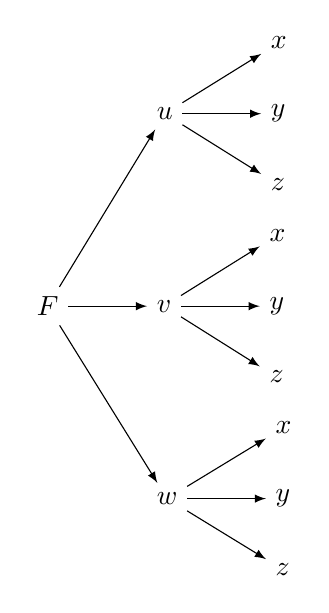
\begin{tikzpicture}[>=latex, baseline=(current bounding box.center)]
\node (F) at (0,0) {$F$};
\node[above right=2cm and 1cm of F] (u) {$u$};
\node[right=2cm and 1cmof F] (v) {$v$};
\node[below right=2cm and 1cmof F] (w) {$w$};
\node[above right=0.5cm and 1cm of u] (x1) {$x$};
\node[above right=0.5cm and 1cm of v] (x2) {$x$};
\node[above right=0.5cm and 1cm of w] (x3) {$x$};
\node[right=0.5cm and 1cm of u] (y1) {$y$};
\node[right=0.5cm and 1cm of v] (y2) {$y$};
\node[right=0.5cm and 1cm of w] (y3) {$y$};
\node[below right=0.5cm and 1cm of u] (z1) {$z$};
\node[below right=0.5cm and 1cm of v] (z2) {$z$};
\node[below right=0.5cm and 1cm of w] (z3) {$z$};
\draw[->] (F) -- (u);
\draw[->] (F) -- (v);
\draw[->] (F) -- (w);
\draw[->] (u) -- (x1);
\draw[->] (v) -- (x2);
\draw[->] (w) -- (x3);
\draw[->] (u) -- (y1);
\draw[->] (v) -- (y2);
\draw[->] (w) -- (y3);
\draw[->] (u) -- (z1);
\draw[->] (v) -- (z2);
\draw[->] (w) -- (z3);
\end{tikzpicture}\qquad$\begin{cases}
\dfrac{\partial F}{\partial x}=\dfrac{\partial f}{\partial u}\cdot\dfrac{\partial u}{\partial x}+\dfrac{\partial f}{\partial v}\cdot\dfrac{\partial v}{\partial x}+\dfrac{\partial f}{\partial w}\cdot\dfrac{\partial w}{\partial x}\\
\dfrac{\partial F}{\partial y}=\dfrac{\partial f}{\partial u}\cdot\dfrac{\partial u}{\partial y}+\dfrac{\partial f}{\partial v}\cdot\dfrac{\partial v}{\partial y}+\dfrac{\partial f}{\partial w}\cdot\dfrac{\partial w}{\partial y}\\
\dfrac{\partial F}{\partial z}=\dfrac{\partial f}{\partial u}\cdot\dfrac{\partial u}{\partial z}+\dfrac{\partial f}{\partial v}\cdot\dfrac{\partial v}{\partial z}+\dfrac{\partial f}{\partial w}\cdot\dfrac{\partial w}{\partial z}\\
\end{cases}$
\end{center}

$\begin{array}{l}
\dfrac{\partial u}{\partial x}=y\cdot x^{y-1}\\
\dfrac{\partial v}{\partial x}=0\\
\dfrac{\partial w}{\partial x}=z^{x}\cdot \ln(z)\\
\dfrac{\partial F}{\partial x}=\dfrac{\partial f}{\partial u}\cdot y\cdot x^{y-1}+\dfrac{\partial f}{\partial w}\cdot z^{x}\cdot\ln(z)
\end{array}$

$\begin{array}{l}
\dfrac{\partial u}{\partial y}=x^{y}\ln(x)\\
\dfrac{\partial v}{\partial y}=z\cdot y^{z-1}\\
\dfrac{\partial w}{\partial y}=0\\
\dfrac{\partial F}{\partial y}=\dfrac{\partial f}{\partial u}\cdot x^{y}\ln(x)+\dfrac{\partial f}{\partial v}\cdot z\cdot y^{z-1}
\end{array}$

$\begin{array}{l}
\dfrac{\partial u}{\partial z}=0\\
\dfrac{\partial v}{\partial z}=y^{z}\ln(y)\\
\dfrac{\partial w}{\partial z}=x\cdot z^{x-1}\\
\dfrac{\partial F}{\partial z}=\dfrac{\partial f}{\partial v}\cdot y^{z}\ln(y)+\dfrac{\partial f}{\partial w}\cdot x\cdot z^{x-1}
\end{array}$

\item \lb{Calcular la expresión de las derivadas parciales de las funciones $F:\R^3\to\R$ dadas por}
\begin{enumerate}[label=\color{red}\textbf{\alph*)}]
	\item $\db{F(x,y,z)=\int_{0}^{x+y+z}\sin t\dt}$
	
	Según la regla de Leibniz, la derivada parcial de $F(x,y,z)$ respecto a cada variable es:
	
	$\begin{array}{l}
	\dfrac{\partial F}{\partial x}=\sin(x+y+z)\cdot\dfrac{\partial (x+y+z)}{\partial x}=\sin(x+z+y)\\
	\dfrac{\partial F}{\partial y}=\sin(x+y+z)\cdot\dfrac{\partial (x+y+z)}{\partial y}=\sin(x+z+y)\\
	\dfrac{\partial F}{\partial z}=\sin(x+y+z)\cdot\dfrac{\partial (x+y+z)}{\partial z}=\sin(x+z+y)\\
	\end{array}$
	\item $\db{F(x,y,z)=\int_{0}^{xyz}t\sin t\dt}$
	
	Según la regla de Leibniz, la derivada parcial de $F(x,y,z)$ respecto a cada variable es:
		
		$\begin{array}{l}
		\dfrac{\partial F}{\partial x}=\sin(xyz)\cdot\dfrac{\partial (xyz)}{\partial x}=\sin(x+z+y)\cdot yz\\
		\dfrac{\partial F}{\partial y}=\sin(xyz)\cdot\dfrac{\partial (xyz)}{\partial y}=\sin(x+z+y)\cdot xz\\
		\dfrac{\partial F}{\partial z}=\sin(xyz)\cdot\dfrac{\partial (xyz)}{\partial z}=\sin(x+z+y)\cdot xy\\
		\end{array}$
	\item $\db{F(x,y,z)=\int_{x^2+y^2}^{xyz}\sin t\dt}$
	
	Según la regla de Leibniz, la derivada parcial de $F(x,y,z)$ respecto a cada variable es:
	
	$\begin{array}{l}
		\dfrac{\partial F}{\partial x}=\sin(xyz)\cdot\dfrac{\partial (xyz)}{\partial x}-\sin(x^2+y^2)\dfrac{\partial(x^2+y^2)}{\partial x}=\sin(x+z+y)\cdot yz-\sin(x^2+y^2)\cdot 2x\\
		\dfrac{\partial F}{\partial y}=\sin(xyz)\cdot\dfrac{\partial (xyz)}{\partial y}-\sin(x^2+y^2)\dfrac{\partial(x^2+y^2)}{\partial y}=\sin(x+z+y)\cdot xz-\sin(x^2+y^2)\cdot 2y\\
		\dfrac{\partial F}{\partial z}=\sin(xyz)\cdot\dfrac{\partial (xyz)}{\partial x}-\tozero{\sin(x^2+y^2)\dfrac{\partial(x^2+y^2)}{\partial z}}=\sin(x+z+y)\cdot xy\\
	\end{array}$
	
\end{enumerate}
	\item \lb{Sea $f:\R\to\R$ una función de clase $C^2(\R,\R)$ y sea $F:\R^2\to\R$ definida por \[ F(x,y)=f\left(\dfrac{1}{y}-\dfrac{1}{x}\right)\text{ con }x,y\neq0. \]Comprobar que se satisfacen las siguientes igualdades:}
	\begin{enumerate}[label=\color{red}\textbf{\alph*)}]
		\item $\db{x^2\dfrac{\partial F}{\partial x}(x,y)+y^2\dfrac{\partial F}{\partial y}(x,y)=0}$
		
		$\begin{array}{l}
		\dfrac{\partial F}{\partial x}=\dfrac{1}{x^2}\\
		\dfrac{\partial F}{\partial y}=-\dfrac{1}{y^2}\\
		\cancel{x^2}\cdot\dfrac{1}{\cancel{x^2}}+\cancel{y^2}\cdot\left(-\dfrac{1}{\cancel{y^2}}\right)=1-1=0
		\end{array}$
		
		\item $\db{xy(x+y)\dfrac{\partial^2 F}{\partial x\partial y}}(x,y)+x^2\dfrac{\partial^2 F}{\partial x^2}(x,y)+y^2\dfrac{\partial^2 F}{\partial y^2}(x,y)=0$
		
		$\begin{array}{l}
		\dfrac{\partial^2 F}{\partial x^2}=\dfrac{\partial }{\partial x}\left(\dfrac{\partial f}{\partial x}\right)=\dfrac{\partial}{\partial x}\left(\dfrac{\partial }{\partial x}\left(\dfrac{1}{y}-\dfrac{1}{x}\right)\right)=\dfrac{\partial }{\partial x}\left(\dfrac{1}{x^2}\right)=-\dfrac{2}{x^3}\\
		\dfrac{\partial^2 F}{\partial y^2}=\dfrac{\partial }{\partial y}\left(\dfrac{\partial f}{\partial y}\right)=\dfrac{\partial}{\partial y}\left(\dfrac{\partial }{\partial y}\left(\dfrac{1}{y}-\dfrac{1}{x}\right)\right)=\dfrac{\partial}{\partial y}\left(-\dfrac{1}{y^2}\right)=\dfrac{2}{y^3}\\
		\dfrac{\partial^2 F}{\partial x\partial y}=\dfrac{\partial }{\partial x}\left(\dfrac{\partial f}{\partial y}\right)=\dfrac{\partial}{\partial x}\left(\dfrac{\partial }{\partial y}\left(\dfrac{1}{y}-\dfrac{1}{x}\right)\right)=\dfrac{\partial}{\partial x}\left(-\dfrac{1}{y^2}\right)=0\\
		\cancel{xy(x+y)\cdot0}+\cancel{x^2}\cdot\left(-\dfrac{2}{x^{\cancel{3}}}\right)+\cancel{y^2}\cdot\dfrac{2}{y^{\cancel{3}}}=-\dfrac{2}{x}+\dfrac{2}{y}\neq0
		\end{array}$
	\end{enumerate}
	\item \lb{Sea $f:\R\to\R$ una función de clase $C^2(\R)$ y sea $F:\R^2\to\R$ definida por \[ F(x,y)=\dfrac{f\left(\frac{y}{x}\right)}{x}\text{ con }x\neq0. \]Comprobar que se satisfacen las igualdades:}
	\begin{enumerate}[label=\color{red}\textbf{\alph*)}]
		\item $\db{x\dfrac{\partial F}{\partial x}(x,y)+y\dfrac{\partial F}{\partial y}(x,y)+F(x,y)=0}$
		
		$\begin{array}{l}
		\dfrac{\partial F}{\partial x}=\dfrac{\partial}{\partial x}\left(\dfrac{f\left(\frac{y}{x}\right)}{x}\right)=\dfrac{x\cdot f'\left(\frac{y}{x}\right)\cdot\left(-\frac{y}{x^2}\right)+\left(\frac{y}{x}\right)\cdot 1}{x^2}=\dfrac{-f'\left(\frac{y}{x}\right)\cdot \frac{y}{x}-f\left(\frac{y}{x}\right)}{x^2}\\
		\dfrac{\partial F}{\partial y}=\dfrac{\partial}{\partial x}\left(\dfrac{f\left(\frac{y}{x}\right)}{x}\right)=\dfrac{1}{x}f'\left(\frac{y}{x}\right)\cdot \dfrac{1}{x}=\dfrac{f'\left(\frac{y}{x}\right)}{x^2}\\
		\begin{aligned}
		\cancel{x}\cdot\left(\dfrac{-f'\left(\frac{y}{x}\right)\cdot \frac{y}{x}-f\left(\frac{y}{x}\right)}{x^{\cancel{2}}}\right)+y\cdot\left(\dfrac{f'\left(\frac{y}{x}\right)}{x^2}\right)+\dfrac{f\left(\frac{y}{x}\right)}{x}&=\dfrac{-f'\left(\frac{y}{x}\right)\cdot\frac{y}{x}-\cancel{f\left(\frac{y}{x}\right)}}{x}+\dfrac{y\cdot f'\left(\frac{y}{x}\right)}{x^2}+\cancel{\dfrac{f\left(\frac{y}{x}\right)}{x}}\\
		&=-\dfrac{f'\left(\frac{y}{x}\right)\cdot y}{x^2}+\dfrac{y\cdot f'\left(\frac{y}{x}\right)}{x^2}=0
		\end{aligned}
		\end{array}$
		
		\item $\db{x^2\dfrac{\partial^2 F}{\partial x^2}(x,y)+y^2\dfrac{\partial^2 F}{\partial y^2}(x,y)+2xy\dfrac{\partial^2 F}{\partial x\partial y}(x,y)=2F(x,y)}$
		
		$\begin{array}{l}
		\dfrac{\partial^2 F}{\partial x^2}=\dfrac{\partial }{\partial x}\left(\dfrac{\partial F}{\partial x}\right)=\dfrac{\partial }{\partial x}\left(\dfrac{-f'\left(\frac{y}{x}\right)\cdot\frac{y}{x}-f\left(\frac{y}{x}\right)}{x^2}\right)=\dfrac{2f''\left(\frac{y}{x}\right)\cdot\frac{y^2}{x^4}+2f'\left(\frac{y}{x}\right)\cdot\frac{y}{x^3}}{x^2}\\
		\dfrac{\partial^2 F}{\partial y^2}=\dfrac{\partial }{\partial y}\left(\dfrac{\partial F}{\partial y}\right)=\dfrac{\partial}{\partial y}\left(\dfrac{f'\left(\frac{y}{x}\right)}{x}\right)=\dfrac{f''\left(\frac{y}{x}\right)}{x^4}\\
		\dfrac{\partial^2 F}{\partial x\partial y}=\dfrac{\partial }{\partial x}\left(\dfrac{\partial F}{\partial y}\right)=\dfrac{\partial }{\partial x}\left(\dfrac{f'\left(\frac{y}{x}\right)}{x}\right)=\dfrac{-f''\left(\frac{y}{x}\right)\cdot\frac{y}{x^3}}{x^2}\\
		
		\end{array}$
	\end{enumerate}
\item \lb{Sea $f(x,y=x^2+y^2)$ y hagmaos $x=\sin t$ e $y=t$ con lo que se obtiene la función compuesta $F(t)=f(x(t), y(t))$. Calcular las tres primeras derivadas de dicha función.}

	Sustituimos $x=\sin t$ y $y=\sin t$ en $f(x,y)=x^2+y^2$: \[F(t)=f(x(t), y(t))=(\sin t)^2+t^2\]
\begin{itemize}
	\item Primera derivada:

	Usamos la regla de la derivada para cada término: 
		\[F'(t)=\dfrac{\partial }{\partial t}(\sin^2t)+\dfrac{\partial}{\partial t}(t^2)=2\cdot\sin t\cdot\cos t+2t\]

	\item Segunda derivada:

	Usamos la regla de la derivada en cada término:

		\[F''(t)=\dfrac{\partial}{\partial t}(2\cdot\sin t\cdot\cos t)+\dfrac{\partial}{\partial t}(2t)=2\cdot\left[\cos t\cdot\cos t+\sin t\cdot (-\sin t)\right]+2=2(\cos^2 t-\sin^2 t)+2\]

	\item Tercera derivada:

		\[F'''(t)=\dfrac{\partial}{\partial t}(2(\cos^2t-\sin^2 t)+\dfrac{\partial }{\partial t}(2)=2\cdot\left(2\cdot\cos t(-\sin t)-2\sin t\cos t\right)+0=-2\cdot(-4\cos t\sin t)=-8\cos t\sin t\]
\end{itemize}

\item \lb{Dada $f(x,y,z)$ se define el gradiente de $f$ como \[\mathrm{grad}f(x,y,z)=\left(\dfrac{\partial f}{\partial x}(x,y,z),\dfrac{\partial f}{\partial y}(x,y,z),\dfrac{\partial f}{\partial z}(x,y,z)\right).\]Dadas las coorenadas cilíndricas de $\R^3$ \[\begin{cases}
x=r\cos\theta\\
y=r\sin\theta\\
z=z
\end{cases}\]obtener el gradiente de $f$ en estas coordenadas.}

\begin{center}
	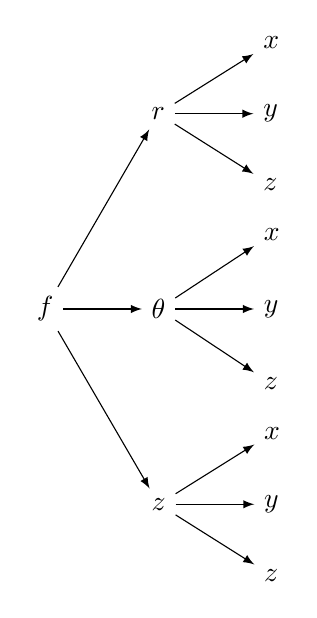
\begin{tikzpicture}[>=latex, baseline=(current bounding box.center)]
		\node (f) at (0,0) {$f$};
		\node[above right=2cm and 1cm of f] (r) {$r$};
		\node[right=2cm and 1cm of f] (t) {$\theta$};
		\node[below right=2cm and 1cm of f] (z) {$z$};
		\node[above right=0.5cm and 1cm of r] (x1) {$x$};
		\node[above right=0.5cm and 1cm of t] (x2) {$x$};
		\node[above right=0.5cm and 1cm of z] (x3) {$x$};
		\node[right=0.5cm and 1cm of r] (y1) {$y$};
		\node[right=0.5cm and 1cm of t] (y2) {$y$};
		\node[right=0.5cm and 1cm of z] (y3) {$y$};
		\node[below right=0.5cm and 1cm of r] (z1) {$z$};
                \node[below right=0.5cm and 1cm of t] (z2) {$z$};
                \node[below right=0.5cm and 1cm of z] (z3) {$z$};
		\draw[->] (f) -- (r);
		\draw[->] (f) -- (t);
		\draw[->] (f) -- (z);
		\draw[->] (r) -- (x1);
		\draw[->] (t) -- (x2);
		\draw[->] (z) -- (x3);
		\draw[->] (r) -- (y1);
		\draw[->] (t) -- (y2);
		\draw[->] (z) -- (y3);
		\draw[->] (r) -- (z1);
		\draw[->] (t) -- (z2);
		\draw[->] (z) -- (z3);
	\end{tikzpicture}\qquad$\begin{cases}
		\dfrac{\partial f}{\partial x}=\dfrac{\partial f}{\partial r}\cdot\dfrac{\partial r}{\partial x}+\dfrac{\partial f}{\partial \theta}\cdot\dfrac{\partial \theta}{\partial x}+\dfrac{\partial f}{\partial z}\cdot\dfrac{\partial z}{\partial x}\\
		\dfrac{\partial f}{\partial y}=\dfrac{\partial f}{\partial r}\cdot\dfrac{\partial r}{\partial y}+\dfrac{\partial f}{\partial \theta}\cdot\dfrac{\partial \theta}{\partial y}+\dfrac{\partial f}{\partial z}\cdot\dfrac{\partial z}{\partial y}\\
		\dfrac{\partial f}{\partial z}=\dfrac{\partial f}{\partial r}\cdot\dfrac{\partial r}{\partial z}+\dfrac{\partial f}{\partial \theta}\cdot\dfrac{\partial \theta}{\partial z}+\dfrac{\partial f}{\partial z}\cdot\lbb{\dfrac{\partial z}{\partial z}}{1}
	\end{cases}$
\end{center}
\begin{enumerate}[label=\arabic*)]
	\item Relación para $r$: \[r=\sqrt{x^2+y^2},\quad\dfrac{\partial r}{\partial x}=\dfrac{x}{\sqrt{x^2+y^2}},\quad\dfrac{\partial r}{\partial y}=\dfrac{y}{\sqrt{x^2+y^2}},\quad\dfrac{\partial r}{\partial z}=0\]
	\item Relación para $\theta$: \[\theta=\tan^{-1}\left(\dfrac{y}{x}\right),\quad\dfrac{\partial \theta}{\partial x}=-\dfrac{y}{x^2+y^2},\quad\dfrac{\partial \theta}{\partial y}=\dfrac{x}{x^2+y^2},\quad\dfrac{\partial \theta}{\partial z}=0\]
	\item Relación para $z$: \[z=z,\quad\dfrac{\partial z}{\partial x}=0,\quad\dfrac{\partial z}{\partial y}=0,\quad\dfrac{\partial z}{\partial z}=1\]

\textbf{Graiente en coordenadas cilíndricas:}

		El gradiente en coordenadas cilíndricas se expresa como: \[\mathrm{grad}f(r,\theta,z)=\left(\dfrac{\partial f}{\partial r},\dfrac{1}{r}\cdot\dfrac{\partial f}{\partial \theta},\dfrac{\partial f}{\partial z}\right)\]

		Derivamos cada componente de $f(x,y,z)$ respecto a $(r,\theta,z)$:

		\begin{enumerate}[label=\arabic*)]
			\item Derivada respecto a $r$: \[\dfrac{\partial f}{\partial r}=\dfrac{\partial f}{\partial x}\dfrac{\partial x}{\partial r}+\dfrac{\partial f}{\partial z}\tozero{\dfrac{\partial z}{\partial r}}=\dfrac{\partial f}{\partial x}\cos\theta+\dfrac{\partial f}{\partial y}\sin\theta\]
			\item Derivada respecto a $\theta$: \[\dfrac{\partial f}{\partial \theta}=\dfrac{\partial f}{\partial x}\dfrac{\partial x}{\partial \theta}+\dfrac{\partial f}{\partial y}\dfrac{\partial y}{\partial \theta}+\dfrac{\partial f}{\partial z}\tozero{\dfrac{\partial z}{\partial \theta}}=\dfrac{\partial f}{\partial x}(-r\sin\theta)+\dfrac{\partial f}{\partial y}(r\cos\theta)\]

			\item Derivada respecto a $z$
				\[\dfrac{\partial f}{\partial z}=\dfrac{\partial f}{\partial x}\tozero{\dfrac{\partial x}{\partial z}}+\dfrac{\partial f}{\partial y}\tozero{\dfrac{\partial y}{\partial z}}+\dfrac{\partial f}{\partial z}\dfrac{\partial z}{\partial z}=\dfrac{\partial f}{\partial z}\]
		\end{enumerate}
\end{enumerate}

\item \lb{Si ahora tenemos las coordenadas esféricas \[
		\begin{cases}
			x=r\cos\theta\sin\varphi\\
			y=r\sin\theta\sin\varphi\\
			z=r\cos\varphi
		\end{cases}
	\]obtener el gradiente de la función del ejercicio anterior en estas nuevas coordenadas.} 

El gradiente de $f$ en coordenadas cartesianas es: \[\mathrm{grad}f(x,y,z)=\left(\dfrac{\partial f}{\partial x},\dfrac{\partial f}{\partial y},\dfrac{\partial f}{\partial z}\right).\]
Queremos expresar este gradiente en términos de coordenadas esféricas $(r,\theta,\varphi)$.

\begin{enumerate}[label=\arabic*)]
\item Relación entre derivadas parciales

Usamos la regla de la cadena para expresar las derivadas parciales respecto a $(x,y,z)$ en términos de $(r,\theta,\varphi)$. Por la regla de la cadena:

\[
\begin{array}{l}
\dfrac{\partial f}{\partial r}=\dfrac{\partial f}{\partial x}\dfrac{\partial x}{\partial r}+\dfrac{\partial f}{\partial y}\dfrac{\partial y}{\partial r}+\dfrac{\partial f}{\partial z}\dfrac{\partial z}{\partial r}\\

\dfrac{\partial f}{\partial \theta}=\dfrac{\partial f}{\partial x}\dfrac{\partial x}{\partial \theta}+\dfrac{\partial f}{\partial y}\dfrac{\partial y}{\partial \theta}+\dfrac{\partial f}{\partial z}\dfrac{\partial z}{\partial \theta}\\

\dfrac{\partial f}{\partial \varphi}=\dfrac{\partial f}{\partial x}\dfrac{\partial x}{\partial \varphi}+\dfrac{\partial f}{\partial y}\dfrac{\partial y}{\partial \varphi}+\dfrac{\partial f}{\partial z}\dfrac{\partial z}{\partial \varphi}\\
\end{array}
\]
\item Gradiente en coordenadas esféricas.

\[
\begin{array}{l}
\dfrac{\partial f}{\partial r}=\dfrac{\partial f}{\partial x}\cos\theta\sin\varphi+\dfrac{\partial f}{\partial y}\sin\theta\sin\varphi+\dfrac{\partial f}{\partial z}\cos\theta\\

\dfrac{\partial f}{\partial \theta}=\dfrac{\partial f}{\partial x}(-r\sin\theta\sin\varphi)+\dfrac{\partial f}{\partial y}(r\cos\theta\sin\varphi)+\cancel{\dfrac{\partial f}{\partial z}\cdot0}=r\sin\varphi\left(-\dfrac{\partial f}{\partial x}\sin\theta+\dfrac{\partial f}{\partial y}\cos\theta\right)\\

\dfrac{\partial f}{\partial \varphi}=\dfrac{\partial f}{\partial x}(r\cos\theta\cos\varphi)+\dfrac{\partial f}{\partial y}(r\sin\theta\cos\varphi)+\dfrac{\partial f}{\partial z}(-r\sin\varphi)=r\left[\cos\varphi\left(\dfrac{\partial f}{\partial x}\cos\theta+\dfrac{\partial f}{\partial y}\sin\theta\right)-\dfrac{\partial f}{\partial z}\sin\varphi\right]
\end{array}
\]
\end{enumerate}

\item \lb{Sea $f:\R^2\backslash\{(0,0)\}\to\R$ una función de clase $C^2(\R^2\backslash\{(0,0)\})$. Comprobar que \[\dfrac{1}{x^2+y^2}\left(\dfrac{\partial^2f}{\partial x^2}(x,y)+\dfrac{\partial^2 f}{\partial y^2}(x,y)\right)=4\left(\dfrac{\partial^2 f}{\partial u^2}(u,v)+\dfrac{\partial^2 f}{\partial v^2}(u,v)\right)\]donde $u=x^2-y^2$ y $v=2xy$.}


\end{enumerate}

\begin{center}
\noindent\rule{0.5\textwidth}{0.5pt}
\end{center}

\begin{enumerate}[label=\color{red}\textbf{\arabic*)}, leftmargin=*]
	\item 
\end{enumerate}
\end{document}
